% ICASSP 2027 submission — draft v1 (numbers marked \xx{} pending final runs)
% Compile: pdflatex main && bibtex main && pdflatex main && pdflatex main
\documentclass{article}
\usepackage{spconf,amsmath,amssymb,graphicx,booktabs}
\usepackage[hidelinks]{hyperref}
\renewcommand{\ttdefault}{cmtt}   % 本機 TeX 缺 pcr（Courier）metrics

\newcommand{\xx}[1]{\textbf{#1}}          % placeholder for pending numbers
\newcommand{\method}{UWRD}               % Utility-Weighted Replay Distillation
\def\x{{\mathbf x}}

\title{Remembering Where to Look: Continual Learning of\\ Budgeted Visual Evidence Acquisition}

% ICASSP is double-blind at submission time.
\name{Anonymous ICASSP 2027 submission}
\address{}

\begin{document}
\maketitle

\begin{abstract}
Many vision systems cannot afford to observe everything: an agent must
sequentially choose \emph{where to look} under a hard observation budget, and
only the acquired evidence feeds the downstream predictor. We show that when
such an evidence-acquisition policy is trained on a sequence of tasks, it
suffers a distinct form of catastrophic forgetting---\emph{navigation
forgetting}---that is invisible to standard continual-learning (CL) metrics:
the policy's selections collapse (selection Jaccard
$\xx{0.79}\!\rightarrow\!\xx{0.07}$) long before accuracy drops, because
within-image signal redundancy lets a frozen predictor compensate for degraded
navigation. Tightening the budget removes this compensation and converts
behavioral forgetting into performance forgetting. We formalize the setting
with a causal feature pyramid environment and a navigation-only attribution
protocol on gigapixel whole-slide images (WSI), where coarse features are
always visible but fine evidence is revealed only after a zoom action, and
per-task predictors are frozen so any degradation is attributable to the
policy. Without human viewing trajectories, we supervise the policy by
counterfactual diagnostic gain, and study Utility-Weighted Replay Distillation
as a targeted variant over compressed navigation states. Across two
four-task and two-task TCGA sequences, replay and policy-fidelity distillation
reduce acquisition drift while behavior-level metrics expose forgetting that
accuracy alone misses.
\end{abstract}

\begin{keywords}
continual learning, active perception, evidence acquisition, whole-slide
images, policy distillation
\end{keywords}

\section{Introduction}
\label{sec:intro}

A pathologist does not read a gigapixel slide exhaustively; they skim a
low-magnification overview, zoom into a few suspicious regions, and commit to
a diagnosis once enough evidence is gathered. The same
\emph{budgeted evidence acquisition} pattern appears whenever observation is
costly: visual navigation, remote sensing, video triage, or token selection in
long-context models. Formally, a lightweight policy sequentially selects $K$
observations from a candidate structure; only selected evidence is revealed
and aggregated for a downstream predictor.

This paper asks what happens to such a policy under \emph{continual learning}
(CL). CL research has focused almost exclusively on classifier forgetting:
representations and decision boundaries drift when tasks arrive sequentially
\cite{kirkpatrick2017ewc,li2017lwf,rebuffi2017icarl}. The acquisition policy
--- \emph{where to look} --- is a separate learned capability, and we show its
forgetting is (i) real and severe, (ii) mechanistically distinct from
prediction forgetting, and (iii) systematically \emph{masked} by signal
redundancy: when many regions carry correlated evidence, a damaged policy
still lands on ``good enough'' regions and accuracy barely moves, while the
selection behavior itself has collapsed. Under tight budgets ($K{=}1,2$) or
longer task sequences, the compensation disappears and the hidden damage
surfaces as accuracy loss.

We make four contributions. \textbf{(1) Problem \& protocol.} We isolate
navigation forgetting with a \emph{causal feature pyramid} environment
(coarse features always visible; fine evidence revealed only after zoom) and
a \emph{navigation-only attribution} protocol: per-task evaluators are frozen
at task end, so any later change on that task is attributable to the shared
policy. We pair standard CL metrics with behavior-level ones (selection
Jaccard, action-distribution KL drift, selected-evidence utility).
\textbf{(2) Weak supervision without trajectories.} Real navigation
demonstrations are unavailable at scale (no expert viewing logs in TCGA); we
derive per-step supervision from slide-level labels via \emph{counterfactual
diagnostic gain} --- how much adding a candidate's evidence reduces the frozen
evaluator's loss --- and train the policy by distribution imitation.
\textbf{(3) Mitigation.} We analyze Utility-Weighted Replay Distillation
(\method{}) as a targeted variant: old-task decision states are stored as
kilobyte feature tuples, and the new policy is regularized toward the old one
preferentially on high-utility states. Uniform policy-fidelity distillation
remains a strong comparison.
\textbf{(4) Findings.} On four-task (ESCA$\to$LUNG$\to$RCC$\to$BRCA) and
two-task TCGA sequences, sequential fine-tuning collapses selection overlap
($\xx{0.07}$ Jaccard at $K{=}2$) with small accuracy change at large budgets,
while the budget--forgetting interaction supports redundancy masking;
\method{} reduces drift in selected settings (Jaccard $\xx{XX}$, action-KL
$\xx{XX}$), while its relative advantage over policy-fidelity distillation is
budget- and order-dependent.

WSI is our benchmark, not our claim: labels are weak, redundancy is
quantifiable, and the coarse-to-fine structure is native. We make no clinical
claims; the methodology targets any budgeted acquisition policy.

\section{Related Work}
\label{sec:related}

\textbf{Continual learning.} Regularization methods penalize drift of
important parameters \cite{kirkpatrick2017ewc}; distillation constrains
outputs on new data \cite{li2017lwf}; rehearsal replays stored exemplars
\cite{rebuffi2017icarl,chaudhry2019er}. In computational pathology, ConSlide
\cite{huang2023conslide} studies WSI classification CL with region-based
rehearsal. All of these preserve \emph{predictions}; none measure or preserve
an \emph{acquisition policy}. Our protocol freezes per-task predictors
precisely to separate the two.

\textbf{Attention-based WSI classification.} Multiple-instance learning
aggregates all patches with attention \cite{ilse2018abmil,lu2021clam}; the
model \emph{sees everything} and ranks post hoc. Our setting enforces partial
observability with a hard budget: unobserved evidence never enters the
predictor, which is what makes ``where to look'' a genuine sequential policy.

\textbf{Visual navigation and active perception.} Vision-language navigation
(VLN) learns instruction-conditioned policies over discrete panorama graphs
\cite{anderson2018r2r}; our coarse-to-fine design echoes DUET's dual-scale
planning over topological maps \cite{chen2022duet} and our evidence state
parallels history-aware encoding \cite{chen2021hamt}; recurrent hard
attention dates to glimpse networks \cite{mnih2014ram}. VLN's
\emph{supervision stack}, however, does not transfer: it rests on human
demonstration trajectories and a geometric, task-agnostic success criterion.
Neither exists for WSI --- expert viewing paths do not scale (a recent
benchmark required ten pathologists for 1.8k slides
\cite{pathagentbench2026}), and success is defined only through a
task-specific evaluator that \emph{changes} with each task. Continual VLN
addresses scene-domain shift with ground-truth-trajectory replay
\cite{jeong2025cvln}; task-incremental navigation under weak,
teacher-drifting supervision is unexplored. Training-free WSI agents
\cite{pathagent2026,pathnavigate2026} navigate each slide from scratch
without learning --- they neither accumulate navigation knowledge nor
forget it.

\section{Problem Setting and Protocol}
\label{sec:setting}

\textbf{Environment.} A slide is a two-level feature pyramid with $R$ regions.
Coarse features $F_{\mathrm{low}} \in \mathbb{R}^{R \times d_\ell}$ are always
visible; fine evidence $z_r \in \mathbb{R}^{d_h}$ is revealed only after the
agent zooms into region $r$ (\emph{causal access rule}). An episode runs $K$
steps: at step $t$ the policy $\pi_\theta$ scores unzoomed candidates from
$[F_{\mathrm{low}}[r]; E_t; b_t]$, where the evidence state
$E_t$ is the mean of revealed fine features and $b_t$ the remaining budget;
the chosen region's $z_{a_t}$ is revealed and aggregated. After $K$ steps a
task evaluator $f$ predicts from $E_K$ alone --- unobserved evidence never
reaches the predictor.

\textbf{Continual protocol.} Tasks $T_1,\dots,T_n$ (disjoint diagnostic
problems) arrive sequentially. A \emph{single shared} navigator is updated
throughout; each task's evaluator $f_j$ is trained within its task and then
\textbf{frozen}. Evaluating task $j$ at any later time uses the frozen $f_j$,
so performance change on $T_j$ is attributable to navigation behavior alone.
We report balanced accuracy, average accuracy (AA), forgetting, and BWT,
plus three behavior-level measurements: \emph{selection Jaccard} between the
regions chosen at task-$j$ time and at sequence end; \emph{action KL drift}
on frozen probe states; and \emph{selected-evidence utility} under $f_j$.

\section{Method}
\label{sec:method}

\textbf{Stage A: evaluator.} $f$ is trained on random $K$-subset evidence
$\bar z_S$, $S\!\sim\!\text{Unif}$, with cross-entropy; the randomization
makes $f$ agnostic to \emph{which} policy produced the evidence, enabling fair
comparison of policies under a frozen $f$.

\textbf{Stage B: counterfactual teacher.} With $f$ frozen, define for
evidence set $E$ and candidate $r$
\begin{equation}
\mathrm{gain}(r \mid E) = \mathrm{CE}\!\big(f(E), y\big) -
\mathrm{CE}\!\big(f(E \cup \{r\}), y\big),
\label{eq:gain}
\end{equation}
the counterfactual reduction in diagnostic loss if $r$ were added. A greedy
rollout produces teacher states with full gain distributions --- per-step
supervision synthesized purely from slide-level labels.

\textbf{Stage C: policy imitation.} The navigator minimizes
\begin{equation}
\mathcal{L}_{\mathrm{nav}} =
\mathrm{KL}\!\big(q \,\|\, \pi_\theta(\cdot \mid s)\big),\quad
q_r \propto \exp\!\big(\mathrm{gain}(r \mid E)/\tau\big),
\label{eq:imit}
\end{equation}
matching the full utility distribution rather than the argmax, which
preserves ranking information on near-tied candidates.

\textbf{CL mechanism (\method{}).} At the end of each task we store, per
training slide, $m$ compressed teacher states
$s=(F_{\mathrm{low}}, E, b, \mathrm{gain}, u)$ --- kilobytes each, no raw
image --- with utility $u(s) = \max_r \mathrm{gain}(r \mid E_s)$. While
learning task $t{+}1$ we optimize
\begin{equation}
\mathcal{L} = \mathcal{L}_{\mathrm{nav}}^{\mathrm{new}}
+ \sum_{s \in \mathcal{M}} \Big[
\mathrm{KL}\big(q_s \| \pi_\theta\big)
+ \lambda\, w(s)\,
\mathcal{L}_{\mathrm{distill}}(s) \Big],\quad
\mathcal{L}_{\mathrm{distill}}(s) = \mathrm{KL}\big(\pi_{\mathrm{old}} \| \pi_\theta\big),
\label{eq:cl}
\end{equation}
with $w(s) = u(s)/\bar u$ clipped at $5$: replayed teacher targets keep the
policy competent on old states, and the distillation term anchors the current
policy $\pi_\theta$ to the old policy $\pi_{\mathrm{old}}$ \emph{most strongly
where evidence choice mattered most}. States whose gain landscape is flat
consume almost no preservation capacity. We write the training-time term
$\mathcal{L}_{\mathrm{distill}}$ and the measurement-time \emph{action-KL
drift} metric with distinct symbols to avoid conflating them: the metric
reported in Table~\ref{tab:main} is
$D_{\mathrm{drift}}(j) = \mathrm{KL}\big(\pi^{(j)}_{\mathrm{own}} \|
\pi_{\mathrm{final}}\big)$, the divergence from task $T_j$'s own-time policy
$\pi^{(j)}_{\mathrm{own}}$ to the sequence-final policy $\pi_{\mathrm{final}}$
on $T_j$'s frozen probe states --- it is never optimized, only measured.

\section{Experiments}
\label{sec:exp}

\textbf{Datasets and sequences.} \emph{Four-task}: TCGA ESCA (ESCC/ESAD,
150 slides) $\to$ LUNG (LUAD/LUSC, 965) $\to$ RCC (CCRCC/PRCC/CHRCC, 888)
$\to$ BRCA (IDC/ILC, 952), CONCH patch features \cite{lu2024conch};
regions are per-slide feature clusters ($R{=}32$), fine evidence is the
cluster mean (512-d), and the coarse view is a fixed lossy 64-d random
projection --- mirroring how a thumbnail is a lossy downsample of the full
image. Patient-level train/val/test splits are fixed; both task orders are
run. \emph{Two-task hierarchy}: a 40-slide renal$\to$breast sequence with
true spatial regions (HIPT \cite{chen2022hipt} coarse, CONCH fine) checks
that findings transfer to a spatial-pyramid environment.
$K \in \{1,2,4\}$, 5 seeds.

\textbf{Baselines.} Sequential fine-tuning (seqft), EWC
\cite{kirkpatrick2017ewc}, LwF-style policy distillation on new-task states
\cite{li2017lwf}, counterfactual-teacher replay, old-policy /
policy-fidelity distillation, replay plus uniform policy distillation,
\method{}, and a joint-training reference. The reference is not treated as an
upper bound. All share the identical frozen-evaluator protocol.

\textbf{Single-task sanity (learnability).} The learned navigator beats
random and spatial-uniform selection at small budgets on both environments
(paired bootstrap 95\% CI excludes 0 for $K\in\{\xx{1,2}\}$;
Fig.~\ref{fig:budget}, left inset), and a full-information linear probe
confirms the features support the tasks. Navigation is learnable and
non-trivial before any CL is attempted.

\begin{figure}[t]
\centering
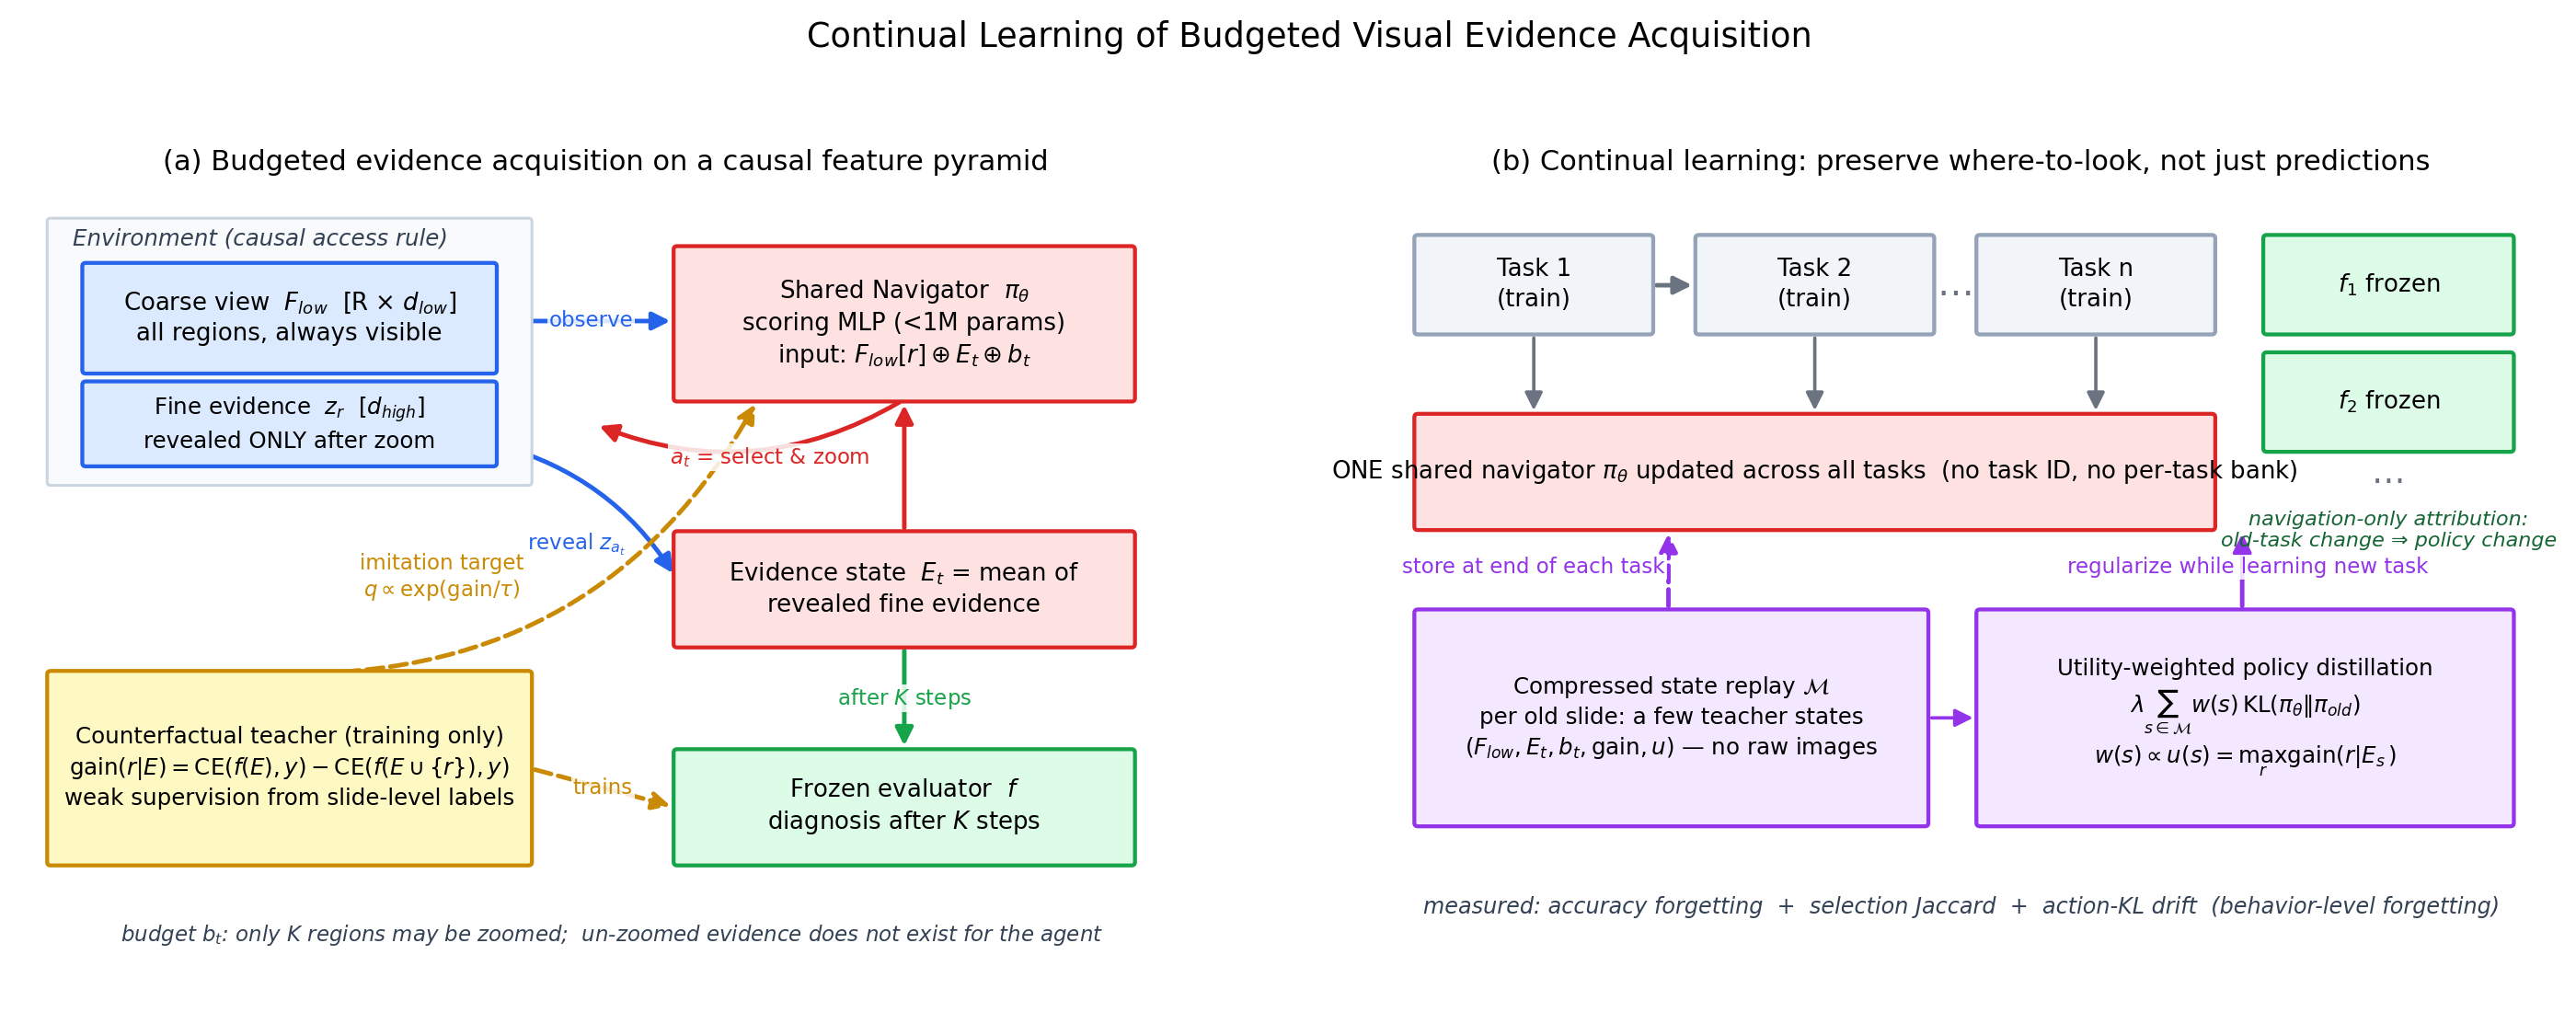
\includegraphics[width=\linewidth]{../figures/fig1_architecture.png}
\caption{\textbf{(a)} Causal feature pyramid: coarse always visible, fine
evidence revealed only on zoom; a counterfactual teacher converts slide-level
labels into per-step supervision. \textbf{(b)} CL loop: frozen per-task
evaluators give navigation-only attribution; \method{} preserves high-utility
acquisition behavior via compressed states.}
\label{fig:arch}
\end{figure}

\textbf{Main result: masked forgetting surfaces under budget pressure.}
Table~\ref{tab:main} reports the four-task sequence.
With seqft, selection Jaccard on $T_1$ collapses to $\xx{0.07}$ and action-KL
drifts by $\xx{XX}$, yet balanced accuracy barely moves at $K{=}4$
($\xx{XX}$): redundancy lets the frozen evaluator compensate. At $K{=}1$--$2$
the compensation weakens and forgetting becomes visible in accuracy
($\xx{XX}$ at $K{=}1$). \method{} reduces forgetting relative to sequential
fine-tuning in the reported settings, but policy-fidelity distillation remains
competitive or better on several behavior metrics. The joint-training
comparison is descriptive, not an upper-bound claim.

\begin{table}[t]
\centering
\caption{Four-task TCGA sequence (main order), mean over 5 seeds.
AA/Forg.\ in balanced accuracy; Jac.\ = mean selection Jaccard on past tasks
at sequence end. Full table with std and reverse order in supplement.}
\label{tab:main}
\resizebox{\linewidth}{!}{%
\begin{tabular}{l ccc ccc}
\toprule
& \multicolumn{3}{c}{$K=1$} & \multicolumn{3}{c}{$K=4$} \\
\cmidrule(lr){2-4} \cmidrule(lr){5-7}
Method & AA$\uparrow$ & Forg.$\downarrow$ & Jac.$\uparrow$
       & AA$\uparrow$ & Forg.$\downarrow$ & Jac.$\uparrow$ \\
\midrule
seqft            & \xx{--} & \xx{--} & \xx{--} & \xx{--} & \xx{--} & \xx{--} \\
EWC              & \xx{--} & \xx{--} & \xx{--} & \xx{--} & \xx{--} & \xx{--} \\
LwF              & \xx{--} & \xx{--} & \xx{--} & \xx{--} & \xx{--} & \xx{--} \\
Replay           & \xx{--} & \xx{--} & \xx{--} & \xx{--} & \xx{--} & \xx{--} \\
Policy-fidelity distill. & \xx{--} & \xx{--} & \xx{--} & \xx{--} & \xx{--} & \xx{--} \\
\method{} (utility variant) & \xx{--} & \xx{--} & \xx{--} & \xx{--} & \xx{--} & \xx{--} \\
\midrule
Joint reference   & \xx{--} & \xx{--} & \xx{--} & \xx{--} & \xx{--} & \xx{--} \\
\bottomrule
\end{tabular}}
\end{table}

\begin{figure}[t]
\centering
\IfFileExists{../figures/cl_budget_forgetting_can_main.png}{%
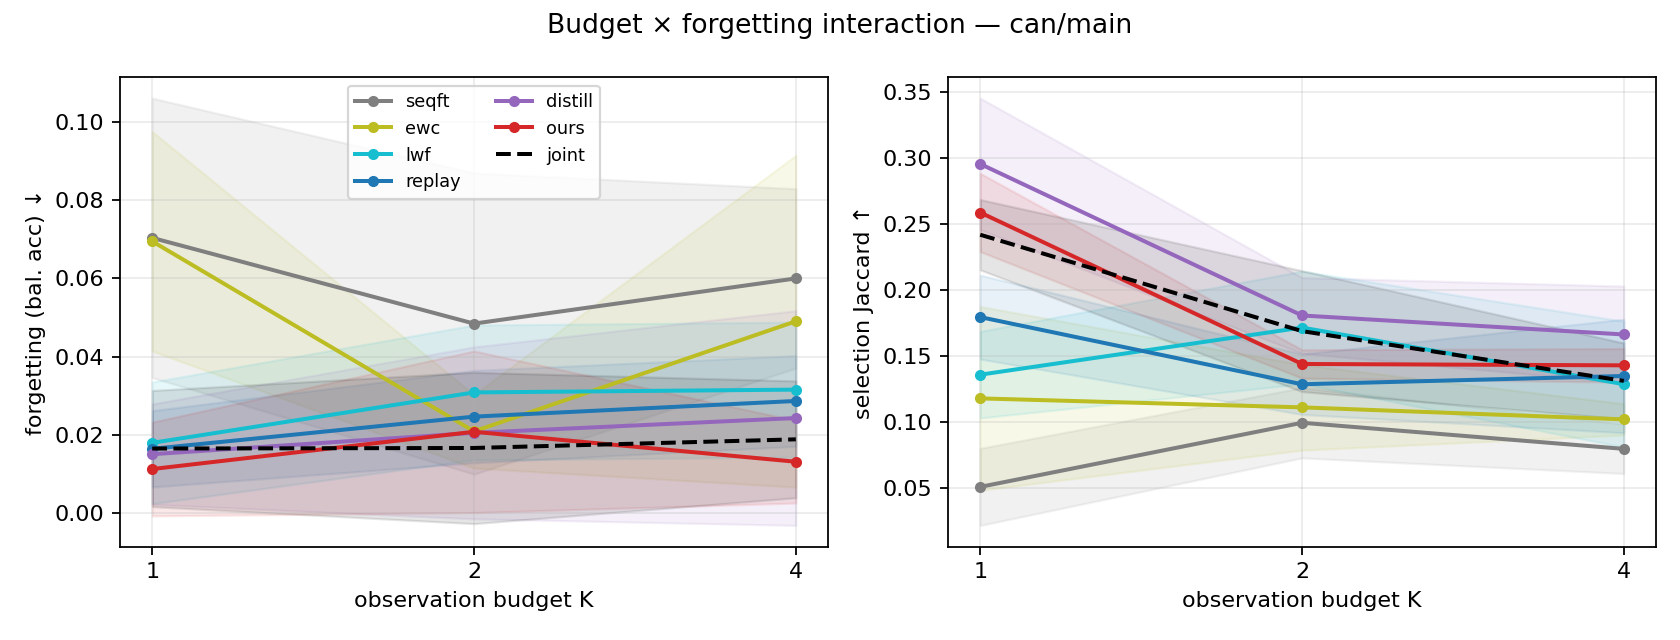
\includegraphics[width=\linewidth]{../figures/cl_budget_forgetting_can_main.png}}{%
\fbox{\parbox[c][3.2cm][c]{0.9\linewidth}{\centering pending: budget--forgetting figure}}}
\caption{Budget--forgetting interaction. Left: accuracy forgetting grows as
the budget tightens (redundancy compensation weakens). Right: selection
Jaccard shows behavior-level forgetting at \emph{all} budgets --- damage that
accuracy metrics miss at large $K$.}
\label{fig:budget}
\end{figure}

\textbf{Mechanism analysis.} (i) \emph{Redundancy masking}: at $K{=}4$,
seqft's selected regions still achieve $\xx{XX}$\% of the counterfactual
utility of task-time selections despite Jaccard $\xx{0.07}$ --- different
regions, similar evidence --- while at $K{=}1$ utility drops to $\xx{XX}$\%,
explaining where accuracy forgetting comes from. (ii) \emph{Utility
weighting}: replacing $w(s)$ with uniform weights changes AA by $\xx{XX}$
and Jaccard by $\xx{XX}$; this is a descriptive mechanism result, not a
universal winner claim. The utility ablation shares utility-prioritized
buffer truncation with the uniform variant, so it isolates distillation-loss
weighting rather than the full effect of utility-aware memory. (iii)
\emph{Memory and $\lambda$}: observed trends are reported as
behavior-fidelity / capability-retention trade-offs and are not universal
monotonic laws.

\section{Conclusion}
\label{sec:conclusion}

Budgeted evidence-acquisition policies forget \emph{where to look} in ways
current CL evaluation cannot see: redundancy hides behavioral collapse until
observation budgets tighten. A frozen-evaluator protocol isolates this
navigation forgetting, counterfactual gain supervises policies without human
trajectories, and Utility-Weighted Replay Distillation is a targeted variant
over compressed states. Limitations: feature-space
pseudo-regions on the four-task benchmark (no public coordinates), mean
evidence aggregation, and fixed budgets; query-conditioned and
dynamic-magnification policies are natural next steps.

\vfill\pagebreak

\bibliographystyle{IEEEbib}
\bibliography{references}

\end{document}
